\chapter{Concept}\label{chapter:concept}
This chapter introduces the architectural design of prototype respect to the previously defined requirements.
Therefore the used development environment will be analyzed.
Followed by the definition of an abstra t architecture of the prototype to be developed.
Based on that the different layer of the system will be elaborated as well as some security concerns and the continuous integration environment.
The working title of the project will be \textbf{Motey}.
In the following the prototype will also be referenced as Motey.


\section{Development environment}
The development environment is crucial for both the implementation of the Motey engine, as well as the choice of possible plugins and libraries.
It should be easy to used and fast to implement, but it should also consider the knowledge of the \ac{FOKUS} as well as the developer.

\paragraph{Java} is still one of the most important programming languages out there.\autocite[cf.]{ProgramminLanguage:2017}
Java is platform indipendent, because Java will not be executed directly in the \ac{OS}, instead it will be executed in the \ac{JVM}.
The downside is, that especially because of the \ac{JVM}, Java programms are much more inefficient regarding \ac{RAM} and \ac{CPU} usage.
Java is object oriented, which makes it easy to extend.
There are a lot of well designed and developed establised libraries and tools out there, which makes it easy to create rapid prototypes.

\paragraph{Node.js} is a relativly young programming environment, which was created 2009 by Ryan Dahl and based on the Google JavaScript engine V8.
The V8 engine is written in C++, which makes the language less resources consuming then for example Java.
A programm will be written in JavaScript, but it is also possible to load C or C++ extension.
Node.js is also available for all common \acp{OS}.
Due to the fact that Node.js has a build-in webserver componant, it is easy to create web applications.
Libraries can be added via the package manager called npm.
JavaScript and also Node.js have a pretty active community, which tends to be as messy as they is increasing.
There is enormous amount of libraries and tools out there, where each library has its reason to exist, but it is also a vast of pretty similar designs and use-cases.

\paragraph{Python} is one of the most used programming languages with a huge and active community.\autocite[cf.]{ProgramminLanguage:2017}
It is a dynamic typed programming language with an automatic memory management which uses both, reference counting and garbage collection at the same time.\autocite[cf.]{Python:GarbageCollection}
Python can use several programming paradigmns like the object oriented programming or functional programming.
Core philosophy is make it simple, make it beautiful, make it explicit and make it readable.
Currently two versions are maintained in parallel, 2.7 and the newer 3.6.
Due to the fact that a huge codebase is still working with Python 2.x, this version is still under development.\autocite[cf.]{Peterson:PythonReleaseSchedule}
Python has a tremendous amount of libraries which can be installed via the Python package manager called pip\footnote{\url{https://pypi.python.org/pypi/pip}}.
Similar to Node.js Python allows to write C extension.
Finally there are several Python compilers which compiles Python code to other high-level languages like Java, C or JavaScript.

\paragraph{Go} is the new emerging language created by Google and was announced end of 2009.
It follows the traditions of C, but also takes added concepts to create a more modern programming language.
According to their own statements go is expressive, concise, clean, and efficient.\autocite[cf.]{Go:Documentation}
Furthermore it has a garbage collection and run-time reflection, it is fast, statically typed and a compiled language.\autocite[cf.]{Go:Documentation}
Go is used in production by several tools like Docker, Kubernetes and OpenShift.
Downside is that there are not so much libraries out right now and there are no long time experience in the critical mass.

Open Baton, as one of the actively maintained project at the \ac{FOKUS}, is written in Java and is also has ports to Python and go.
Python in general is used for several projects at the \ac{FOKUS}.
Taking also the criterias from section \ref{section:functional-requirements} into account Python will be used as the  programming environments of choice.
The \ac{GUI} will only be a very basic web client, which uses Vue.js\footnote{\url{https://vuejs.org}} as its main framework and some smaller tools like the pretty famous bootstrap framework.


\section{Architecture of the system}
The overall architecture of the system can be seperated into two levels.
Figure \ref{fig:abstract_architecture_design} will point up the architecture.
The first level is the \textit{centralized fog level}.
This could be for example a cloud server or management node in a fog cluster.
Ideally this level should be implemented with an \ac{MANO} compliant framework.
Hereinafter Open Baton will referred as the tool of choice for that level.
Main function will be the creation of the \ac{NFVI} as well as the deployment of deployment plans for the \acp{NF}.
Open Baton will also have an overview of all existing nodes and can manage and maintain them.

\begin{figure}[H]
    \centering
    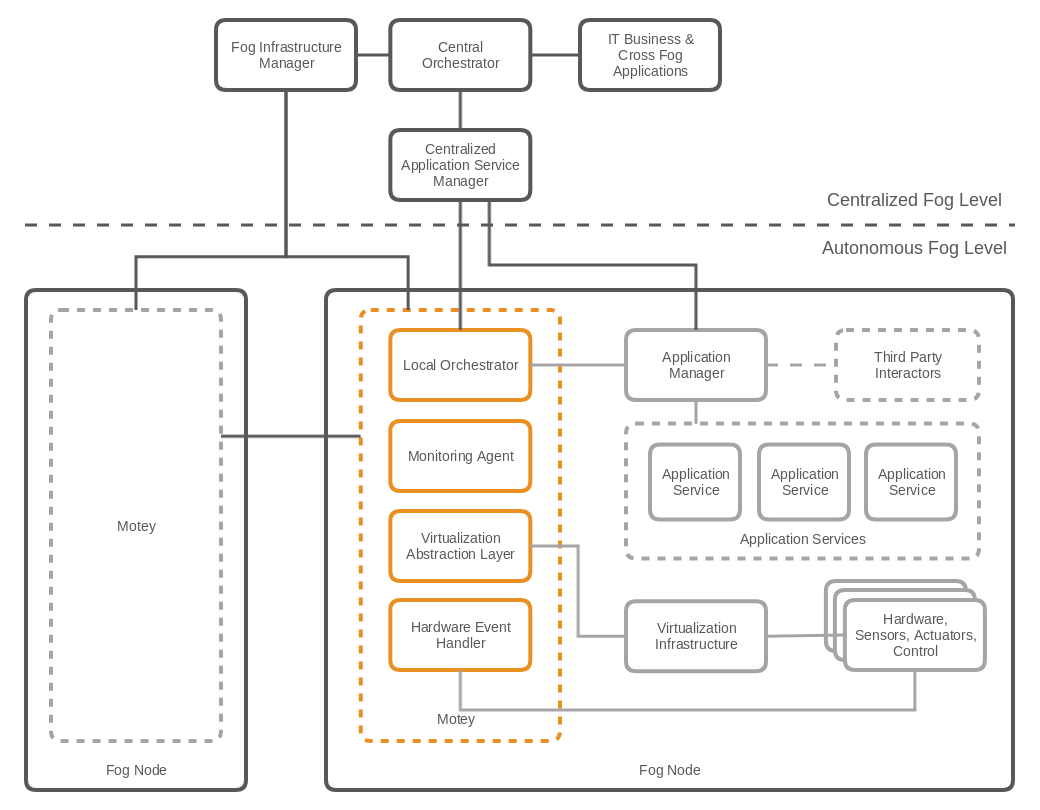
\includegraphics[width=\textwidth]{resources/images/initial_structure.png}
    \caption[Abstract architecture design]{Abstract architecture design}
    \label{fig:abstract_architecture_design}
\end{figure}
% TODO: check if applicaton manager is necessary

The second level is the \textit{autonomous fog level}.
The Motey engine will be located in this level.
It includes all existing fog nodes, as well as the Motey engine that is referenced as the \textit{OpenIoTFog Agent} in figure \ref{fig:abstract_architecture_design}.
Each node must have a running instance of the OpenIoTFog Agent to be part of the system.
Beside Motey a node can have several hardware devices, sensors and actuators connected to them.
A virtualization infrastructure such as Docker or XEN, must be installed to be used by Motey.
These infrastructure can create the containers and \acp{VNF}.
Further it is also possible to have additional third party tools installed which can interact with the them as well.

The OpenIoTFog Agent has several external connection points.
It has a \ac{REST} \ac{API} implemented to get some informations about the status of the fog node, as well as endpoints to receive the deployment plans from centralized fog level.
A \ac{MQTT} connection to a broker, which can be running in the centralized fog level as well as on any other fog node, is used for node discovery.
Finally there are some ZeroMQ endpoints for capability discovery, image deployment and node-to-node communication.
A detailed description will be shown in the following sections.

One of the most important components is the \textit{Local Orchestrator}.
It is responsoible for the deployment of the containers as well as the inter-node communication.
The latter is necessary to let the nodes act in an autonomously was, so that they can react to changing requirements, even when the centralized fog level disappears.
Therefore each node must have knowledge and should be able to interact with each other.
Beside that the local orchestrator is tightly coupled to the \textit{\ac{VAL} Manager}.
This is an abstraction layer for each virtualization component in the system, for example Docker or a bare-metal virtualization like XEN.
These components should be implemented as plugins, so that it is easy to add or remove virtualization components.
Therefore Yapsy\footnote{\url{http://yapsy.sourceforge.net/}} is used as the plugin system of choice.

The \textit{Hardware Event Handler} is a communication endpoint for other third party components.
For example an external hardware listener could send a message to the event handler to register a new connected device like a Zigbee dongle or a bluetooth stick.
This component should allow multiple third party components to send events to them.
Finally the \textit{Monitoring Agenct} is used to log all ongoing events and gives the maintainer of the system an overview of the system processes.

As mentioned in the requirements section \ref{section:functional-requirements} the whole system should be modular and easy to extend.
Therefore each layer will be as decoupled as possible.
A clean architecture with decorated dependencies and only a single responsibility for each component.
The whole code should be independent of any framework, independent of the other components and testable.
To realize such an architecture, multiple design patterns will be used.
\ac{DI} decouple the components and increase the testability.
The decorator pattern will abstract concrete implementations by a centralized independent layer.
The observer pattern can be used to handle streams of data for example from an \ac{API} endpoint.
And finally the singleton pattern can prevent the construction of mulitple instances of a single module.
All of them made the code base well structured and improve the readability as well as the comprehensibility


\subsection{Virtualization layer}
The virtualization layer is basically an abstraction layer to generalize the different virtualization engines.
Therefore a so called \ac{VAL} manager which will be implemented with the facade design pattern is used to load the plugins and abstract the methods of the plugins.
As mentioned before to realize the plugin functionality the Yapsy library will be used.
The library offers a way to easily add new plugins to the system and is also designed to be easy to use.
It only depends on Python standard libraries and lightweight by design.
Each supported virtualization engine needs his own concrete plugin implementation which should be use an interface to have a common ground.
The supported default engine is Docker, but could be extended in a future version of Motey.


\subsection{Communication layer}
\label{subsection:CommunicationLayer}
The communication layer is a pretty important component in the Motey engine.
Here three different communication points are necessary to provide the basic functionalities which are needed for the fog node agent.

The first subcomponent is the \textbf{node discovery}.
The idea behind the node discovery is that each node automatically can register and unregister himself to the cluster.
This means in the moment of the startup of a node, they will send out a message, with an information request about all subscribed nodes.
To realize that \ac{MQTT} will be the tool of choice.
The \ac{MQTT} broker will receive and forward the message to all subscribed nodes and each node will response with an information message to the broker again, which will send the message out again.
Therefore each node will be up-to-date at each time.
As long as there is no appearance or disappearance of any node, the network will not be stressed.
To provide a better flexibility the \ac{MQTT} broker can be executed in the centralized fog level or even on a node in the autonomous fog level.
This allows the system to operate even if the centralized fog level disappears due to network issues or any other communication problems.
It is also possible to let all nodes communicate which each other once they shared their information.
Smaller connection issues can be covered with this mechanism.
As the \ac{MQTT} broker Mosquitto\footnote{\url{https://mosquitto.org}} will be the tool of choice.
It is an eclipse\footnote{\url{http://www.eclipse.org}} project which means it is open source and under continous development.
The project website descibes themself as "a lightweight server implementation of the MQTT protocol that is suitable for all situations from full power machines to embedded and low power machines"\autocite{Eclipse:Mosquitto}.

The next subcomponent is the \textbf{inter- and intra-node communication}.
Both kinds of communication will be realised with ZeroMQ.
Some of the most important patterns and transport types in ZeroMQ was discribed in section \ref{section:ZeroMQ}.
For the node-to-node communication the \textit{Request-Reply} pattern via \ac{TCP} will be used.
Typical function calls would be the capability discovery where a node will request another node for their capabilities, the deployment or termination of an image on an external node and the request for an image status.
ZeroMQ allways requires an \ac{IP} to eastablish a connection to another node, therefore we had the node discovery which was described before.
This allows us to connect to any other node in the cluster.
In addition to the intra-node communication, also an inter-node communication will be implemented.
It will be used to add new capabilities to a node.
Therefore one or multiple third party applications should be connectable to a single ZeroMQ endpoint via the publish/subscribe pattern over \ac{IPC}.
Different to a normal publish/subscribe pattern, the endpoint will acts as the subscriber so that multiple publishers can push messages to them.
Beside that each exposed socket should be configurable via the configuration file.

The last subcomponent is the \textbf{\ac{REST} \ac{API}}.
It will be mainly used for the communication with the centralized fog level, because most of the orchestration tools out there are using \ac{REST} for transfering data.
In comparision to an implementation with ZeroMQ, this is much bigger overhead in terms of traffic and latency, but to have a better compatibility with other systems, this \ac{API} will be implemented.
As the tool of choice Flask\footnote{\url{http://flask.pocoo.org}} will be used.
It is a lightweight and robust Python webserver, which is open source, well documented and under constant development.
The \ac{REST} \ac{API} himself will follow the \ac{HATEOAS} constraint with the addition that each endpoint will have a version number in the \ac{URL} to ensure backwards compatability if something changes in the implementation.

All the mentioned subcomponents should be controlled by a so called \textit{communication manager} which will be implemented with the facade design pattern.
That decouples the communiction layer from the other components, the whole system can be maintained much easier and each subcomponent can be easy replaced by any other technology if necessary.
This also makes the code more readable and leads up to a cleaner code strucutre.


\subsection{Data layer}
As mostly the data layer is used to persist necessary data.
This includes the deployed services, adjacent nodes and the capabilities of the node.
As database engine the lightweight document oriented database TinyDB\footnote{\url{http://tinydb.readthedocs.io}} will be used.
It is easy to use and has no execution overhead and is also good to use for small datasets.
The whole data layer should be as abstracted as all the other components before.
Therefore repositories for each content type will facade the tinydb methods and allows the underlaying library, in this case TinyDB, to be replaced easily and
without modifing several classes.
The configuration of the databases should be stored in the global config file as well.


\subsection{Capability Management}
The \textit{Capability Management} is used to create, persist, modify and remove the capabilities of the current node.
As mentioned before all the capabilities will be stored in the data layer via TinyDB.
Furthermore the \textit{Hardware Event Handler} is part of this layer.
It enables the system to get new capabilites from third party apps via a ZeroMQ endpoint.
As mentioned in the \ref{subsection:CommunicationLayer} the endpoint will be implemented as a form of the publish/subscribe pattern and should allow one or multiple publishers to push messages to the handler.
Also internal components like the \ac{VAL} plugins can add new capabilities to the system.


\subsection{Orchestration layer}
As one of the most important layers, the \textit{Orchestration Layer} will be a connector between all the nodes in a cluster and also between multiple components in the Motey engine himself.
Primary it is used to handle the business logic of the deployment of new services.
If a new service will be send to the communication layer it will be forwarded to the orchestration layer and will be parsed there.
Afterwards the service will be validated and finally deployed by the orchestrator.
Additionally it will also check the necessary capabilities for each service image and will search for suitable nodes in the cluster if one or multiple capabilites are not fulfilled.
Beside that, the orchestrator will also handle the lifecycle of a service and the related images during the deployment phase.
Figure \ref{fig:lifecycle_mgm_squence_diagram_start_service} show up the lifecycle management of a service from the starting phase to the execution phase.

\begin{figure}[H]
    \centering
    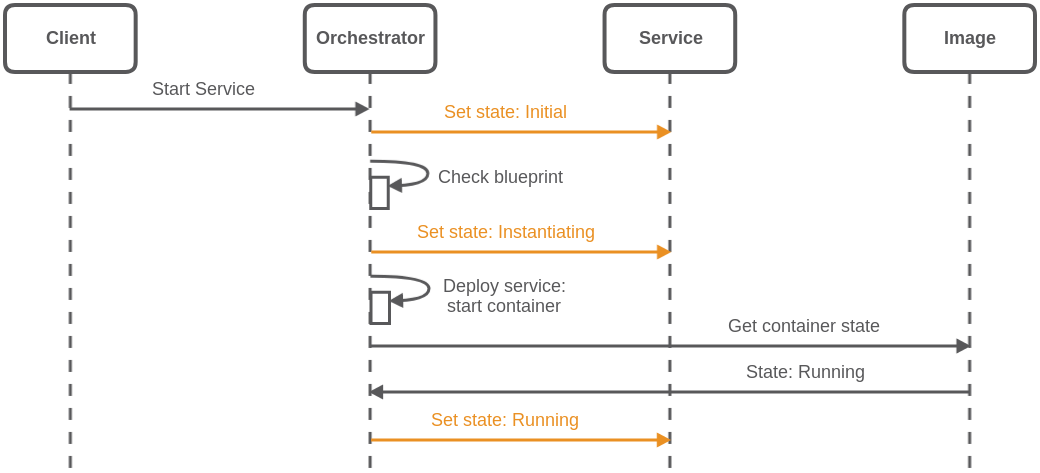
\includegraphics[width=\textwidth]{resources/images/lifecycle_sequence_diagram_start_service.png}
    \caption[Lifecycle management sequence diagram: starting a service]{Lifecycle management sequence diagram: starting a service}
    \label{fig:lifecycle_mgm_squence_diagram_start_service}
\end{figure}

At first a client, for example a webservices via the \ac{REST} \ac{API}, will start a service.
Therefore the related service blueprint will be uploaded to the node.
The orchestrator will directly start with the lifecycle management by creating an service with an \textit{inital} state.
Afterwards the blueprint gets checked by the orchestrator.
If it is not valid, the state of the service would be set to \textit{error}.
In this case everything went fine and the state changes to \textit{instantiating}.
Next the orchestrator will start the images of the servie.
The state of an image can be requestet at every moment during the lifecycle of a service.
After the request for the container state was send, the state will be send back, for example \textit{running}.
When all images are done loading, the state of the service changes to \textit{running}.

Later on the client probably wants to shut down the service.
This time it send the terminate request to the node.
Again the orchestrator will get it and set the state of the service to \textit{stopping}.
Then it will start to shutdown all the related images.
Also in this phase, the state of the images can be requested everytime.
When all images are termianted, the state of the service changes to \textit{terminated} and the service will no longer be executed on the node.
Figure \ref{fig:lifecycle_mgm_squence_diagram_stop_service} illustrates this behavior.

\begin{figure}[H]
    \centering
    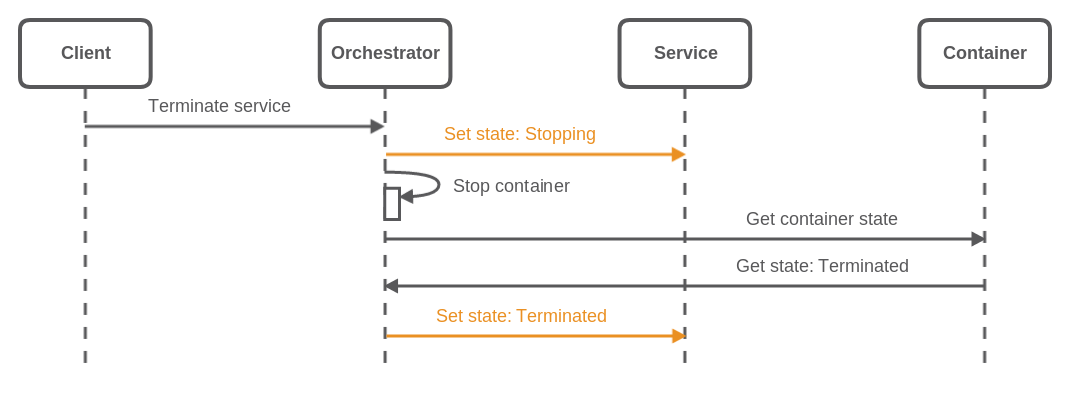
\includegraphics[width=\textwidth]{resources/images/lifecycle_sequence_diagram_stop_service.png}
    \caption[Lifecycle management sequence diagram: stoping a service]{Lifecycle management sequence diagram: stoping a service}
    \label{fig:lifecycle_mgm_squence_diagram_stop_service}
\end{figure}

The lifecycle management of the images is not handled by the orchestrator himself, it will be detected via the lifecycle management of the virtualization engine like Docker or XEN.
Due to the fact that the service is tightly coupled to the images, the state of the images will directly affect the state of the service.
If only one image will change its state to \textit{error} the whole service will be marked as \textit{error}.
To handle the different states of the different engines, a transformation logic between the state will be implemented.


\subsection{User interface}
\doit

\section{Security}
% https://www.golem.de/news/brickerbot-hacker-zerstoeren-das-internet-of-insecure-things-1704-127198.html
% https://www.golem.de/specials/mirai/
% https://www.corero.com/resources/ddos-attack-types/mirai-botnet-ddos-attack.html
% https://www.owasp.org/index.php/OWASP_Internet_of_Things_Project#tab=IoT_Vulnerabilities
% Access control
% Encryption of the communcation channels aka REST, ZeroMQ, MQTT
% Database encryption
\doit


\section{Continuous Integration}
Continuous integration is nowadays a frequently used technique to automate repeating deployment steps into a self executing pipeline.
It starts by running unit tests, code style checks and ends up with deploying the compiled programm to a server or a marktplace.
Due to the fact that Github\footnote{\url{https://github.com}} will be used to host and maintain the git repository for the Motey project, the pretty famous and semless integrated Travis CI\footnote{\url{https://travis-ci.org}} will be used to implement the continuous integration pipeline.
To start with Travis CI only the Github account has to be synced with the platform and a \ac{YAML} configuration file has to be placed in the root folder of the git repository.
Travis CI supports several programming languages and also various third party services, like Docker Hub or Amazon AWS.
Everytime a new commit will be pushed to the git remote repository, a new build will be started at Travis CI.
At first a virtual machine will be started by Travis CI.
Afterwards all necessary components like libraries and tools will be installed in the virtual machine.
Finally all predefined tasks from the \ac{YAML} file will be executed.
In terms of the Motey project, unit tests will be executed, as well as code style checks and if a version from the master branch will be build, a Docker container will be created and pushed to the related Docker Hub repository.
This pipeline guarantees that the project is tested and a coding standard is enforced.
Further the manual build of the Docker container including the upload to the Docker Hub will be obsolete.
